%\documentclass[handout]{beamer}
\documentclass{beamer}
\usepackage{array}
\usepackage{graphicx}
\usepackage{german}
%\usepackage{txfonts}

\mode<beamer>{%
\usetheme[hideothersubsections,hidetitle]{Hannover}
}
\title[]{Partielle Differentialgleichungen}
\subtitle{6. Sitzung: Elliptische PDGL}
\date[25.~M"arz 2015]{25.~M"arz 2015}
\author{Prof.~Dr.~Andreas M"uller}
\begin{document}

\begin{frame}
\section{Elliptische PDGL}
\titlepage
\end{frame}

\begin{frame}
\frametitle{Klassifikation}

\begin{center}
\begin{tabular}{llll}
Klasse&Bedingung&Beispiel&Anwendung\\
\hline
elliptisch &$\begin{aligned}P&=n\mathstrut\end{aligned}$
	&$\displaystyle \Delta u=f                                $
		&Potential\\
&	&	&Eigenwertproblem\\
\hline
parabolisch&%$P=n-1, Z=1$
$\begin{aligned}P&=n-1\mathstrut\\Z&=1\mathstrut\end{aligned}$
	&$\displaystyle \frac{\partial u}{\partial t}=\Delta u    $
		&W"armeleitung\\
\hline
hyperbolisch&%$P=n-1, N=1$
$\begin{aligned}P&=n-1\mathstrut\\N&=1\mathstrut\end{aligned}$
	&$\displaystyle \frac{\partial^2 u}{\partial t^2}=\Delta u$
		&Wellen\\
\hline
\end{tabular}
\end{center}

Klasse verr"at:
\begin{itemize}
\item Charakter der L"osung: Schwingungen, exponentielles Abklingen
\item Welches L"osungsverfahren geeignet ist
\end{itemize}

\end{frame}

\begin{frame}
\frametitle{Problem}
Differentialgleichung
\[
\Delta u=f\qquad\text{in $\Omega$}
\]
Randbedingungen
\[
u_{|\partial \Omega}=g\qquad\text{auf $\partial\Omega$}
\]
\pause
Allgemeine L"osung:
\begin{align*}
u&=u_h+u_p&&\text{mit}&             \Delta u_h&=0,&             \Delta u_p&=f\\
 &        &&          &{u_h}_{|\partial\Omega}&=0,&{u_p}_{|\partial\Omega}&=g
\end{align*}
\begin{enumerate}
\item L"osung existiert $\Leftrightarrow \exists u_p$  
\item Eindeutigkeit der L"osung: $u_h=0$
\end{enumerate}
\end{frame}

\begin{frame}
\frametitle{Maximumprinzip}
\begin{definition}
$u\colon\Omega\to\mathbb R$ heisst harmonisch wenn $\Delta u=0$.
\end{definition}

\pause

\begin{theorem}
Wenn $\Omega$ beschr"ankt und zusammenh"anged ist, dann nimmt eine
harmonische Funktion ihr Maximum und Minimum auf dem Rand $\partial\Omega$ an.
\end{theorem}

\pause

\begin{theorem}
Wenn $\Omega$ beschr"ankt und zusammenh"angend ist, dann ist die 
L"osung des Randwertproblems eindeutig, falls sie existiert.
\end{theorem}

\end{frame}

\begin{frame}
\frametitle{Mittelwerteigenschaft}

\begin{theorem}
Ist $u$ eine harmonische Funktion im Gebiet $\Omega$, dann hat $u$ die
Mittelwerteigenschaft:
\[
u(x)= \int_{S_r(x)}u(\xi)\,d\xi,
\]
wobei $S_r(x)$ eine Kugel mit Radius $r$ um den Punkt $x$ ist, die ganz
in $\Omega$ enthalten ist.
\end{theorem}

{\bf Achtung:} Gilt nur f"ur den gew"ohnlichen Laplace-Operator

\end{frame}

\begin{frame}
\frametitle{Greensche Funktion}
{\bf Problem:}
\begin{align*}
y''(x)&=f(x) \qquad\text{f"ur $x \in (0,1)$}\\
y(0)&=a\\
y(1)&=b
\end{align*}
{\bf Idee:} Gibt es einen inversen Operator der zweiten Ableitung?
\pause
Sieht aus wie eine Matrix
\[
y = \Delta^{-1}f,
\qquad
y(x)=\int_0^1 K(x,\xi)f(\xi)\,d\xi
\]
\pause
{\bf L"osung:} der sog.~Greenschen Funktion $G$:
\[
y(x)=\underbrace{\int_0^1 G(x,\xi)f(\xi)\,d\xi}_{u_p}
+
\underbrace{a(1-x) + bx}_{u_h}
\]
\end{frame}

\begin{frame}
\frametitle{Greensche Funktion}
\begin{align*}
G(x,\xi)
&=
\begin{cases}
(x-\xi) + x(1-\xi) = \xi(x - 1)&\qquad x\ge \xi\\
x(\xi-1)&\qquad x<\xi
\end{cases}
\end{align*}
\end{frame}

\begin{frame}
\frametitle{Greensche Funktion}
\includegraphics[width=\hsize]{../../skript/images/green-1.png}
\end{frame}

\begin{frame}
\frametitle{Greensche Funktion}
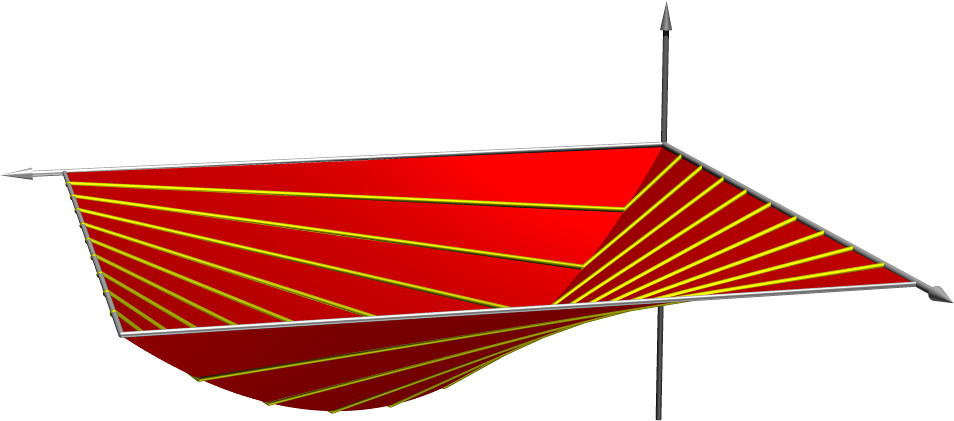
\includegraphics[width=\hsize]{../../skript/3d/green.jpg}
\end{frame}

\begin{frame}
\frametitle{Greensche Funktion}
\includegraphics[width=\hsize]{../../skript/graphics/green-1.pdf}
\end{frame}

\begin{frame}
\frametitle{Greensche Funktion}
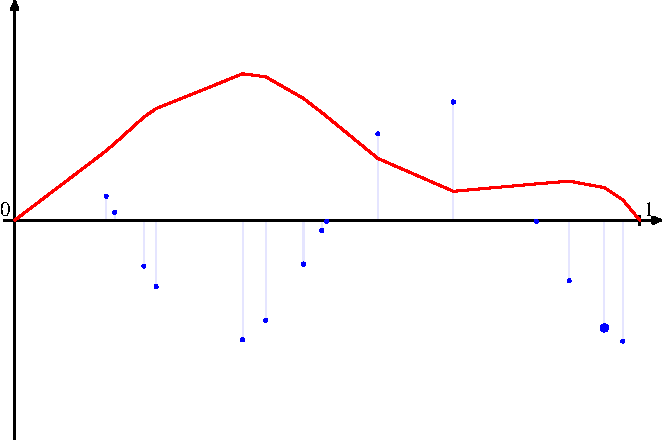
\includegraphics[width=\hsize]{../../skript/graphics/green-324.pdf}
\end{frame}

\begin{frame}
\frametitle{Greensche Funktion}
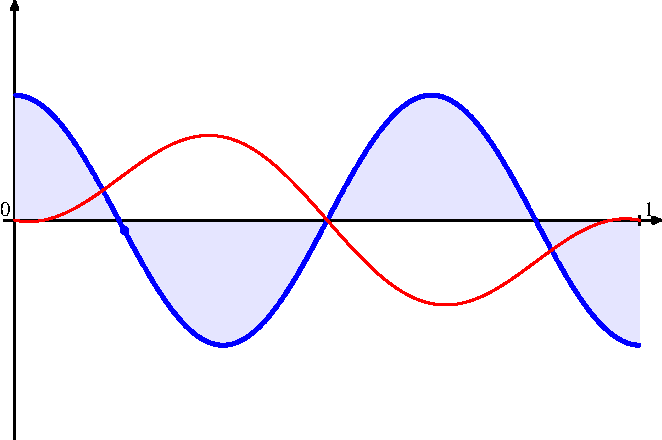
\includegraphics[width=\hsize]{../../skript/graphics/green-1082.pdf}
\end{frame}

\begin{frame}
\frametitle{Greensche Funktion}
Alternative Konstruktion der Greenschen Funktion
\begin{enumerate}[<+->]
\item Einheits-``Knick'':
\[
\sigma(x,\xi)=\frac12|x-\xi|\qquad\text{erf"ullt}\qquad \Delta\sigma(x,\xi)=\delta(x-\xi)
\]
\item harmonische Funktion $h(x,\xi)$ mit gleichen Randwerten:
\[
h(x,\xi)=(1-x)\sigma(0,\xi) + x\sigma(1,\xi)
\]
\item Greensche Funktion:
\[
G(x,\xi) = \sigma(x,\xi) - h(x,\xi)
\]
\end{enumerate}
\pause
Vorteile:
\begin{itemize}[<+->]
\item
$\sigma(x,\xi)$ gibt es in jeder Dimension
\item
Man muss ``nur'' das Problem l"osen
\[
\Delta h = 0, \qquad h_{|\partial\Omega}=\sigma
\]
\end{itemize}
\end{frame}


\begin{frame}
\frametitle{Greensche Funktion}
{\bf Problem:}
\[
\Delta u=f\quad\text{in $\Omega$},\qquad u_{|\partial\Omega}=g
\]
\bigskip

{\bf Idee:} Gibt es einen inversen Operator des Laplace-Operators?
\bigskip

\pause
{\bf Erwartete Form:} Integraloperator
\[
u(x)=\int_\Omega K(x,\xi)f(\xi)\,d\xi
\]
\medskip

\pause
{\bf L"osung:}
\[
u(x)
=
\int_{\Omega} G(x,\xi)f(\xi)\,d\xi
+
\int_{\partial\Omega}  \operatorname{grad}_\xi G(x,\xi) g(\xi)\,d\xi.
\]

\end{frame}

\begin{frame}
\frametitle{Greensche Funktion}

\begin{enumerate}[<+->]
\item
Es gibt eine L"osung $\sigma(x,\xi)$
\[
\Delta \sigma (x,\xi)=\delta(x-\xi)
\]
\item 
Es gibt eine harmonische Funktion $h(x,\xi)$ mit
\[
h(x,\xi)=\sigma(x,\xi),\quad x\in\partial\Omega.
\]
\item
Es gibt eine Funktion
\[
G(x,\xi) = \sigma(x,\xi)-h(x,\xi),
\]
die L"osung des folgenden Randwertproblems ist:
\[
\Delta_x G(x,\xi) = \delta(x-\xi)\quad\text{in $\Omega$},
\qquad
G(x,\xi)=0\quad\text{f"ur $x\in\partial\Omega$}
\]
\end{enumerate}
\end{frame}

\end{document}
